\section{Introduction}

%\begin{enumerate}
%  \item an analysis of the ParSplice keyspace
%  \item using a modern distributed key-value store
%  \item positive effects of Mantle 
%\end{enumerate}

\begin{figure}[t]
  \noindent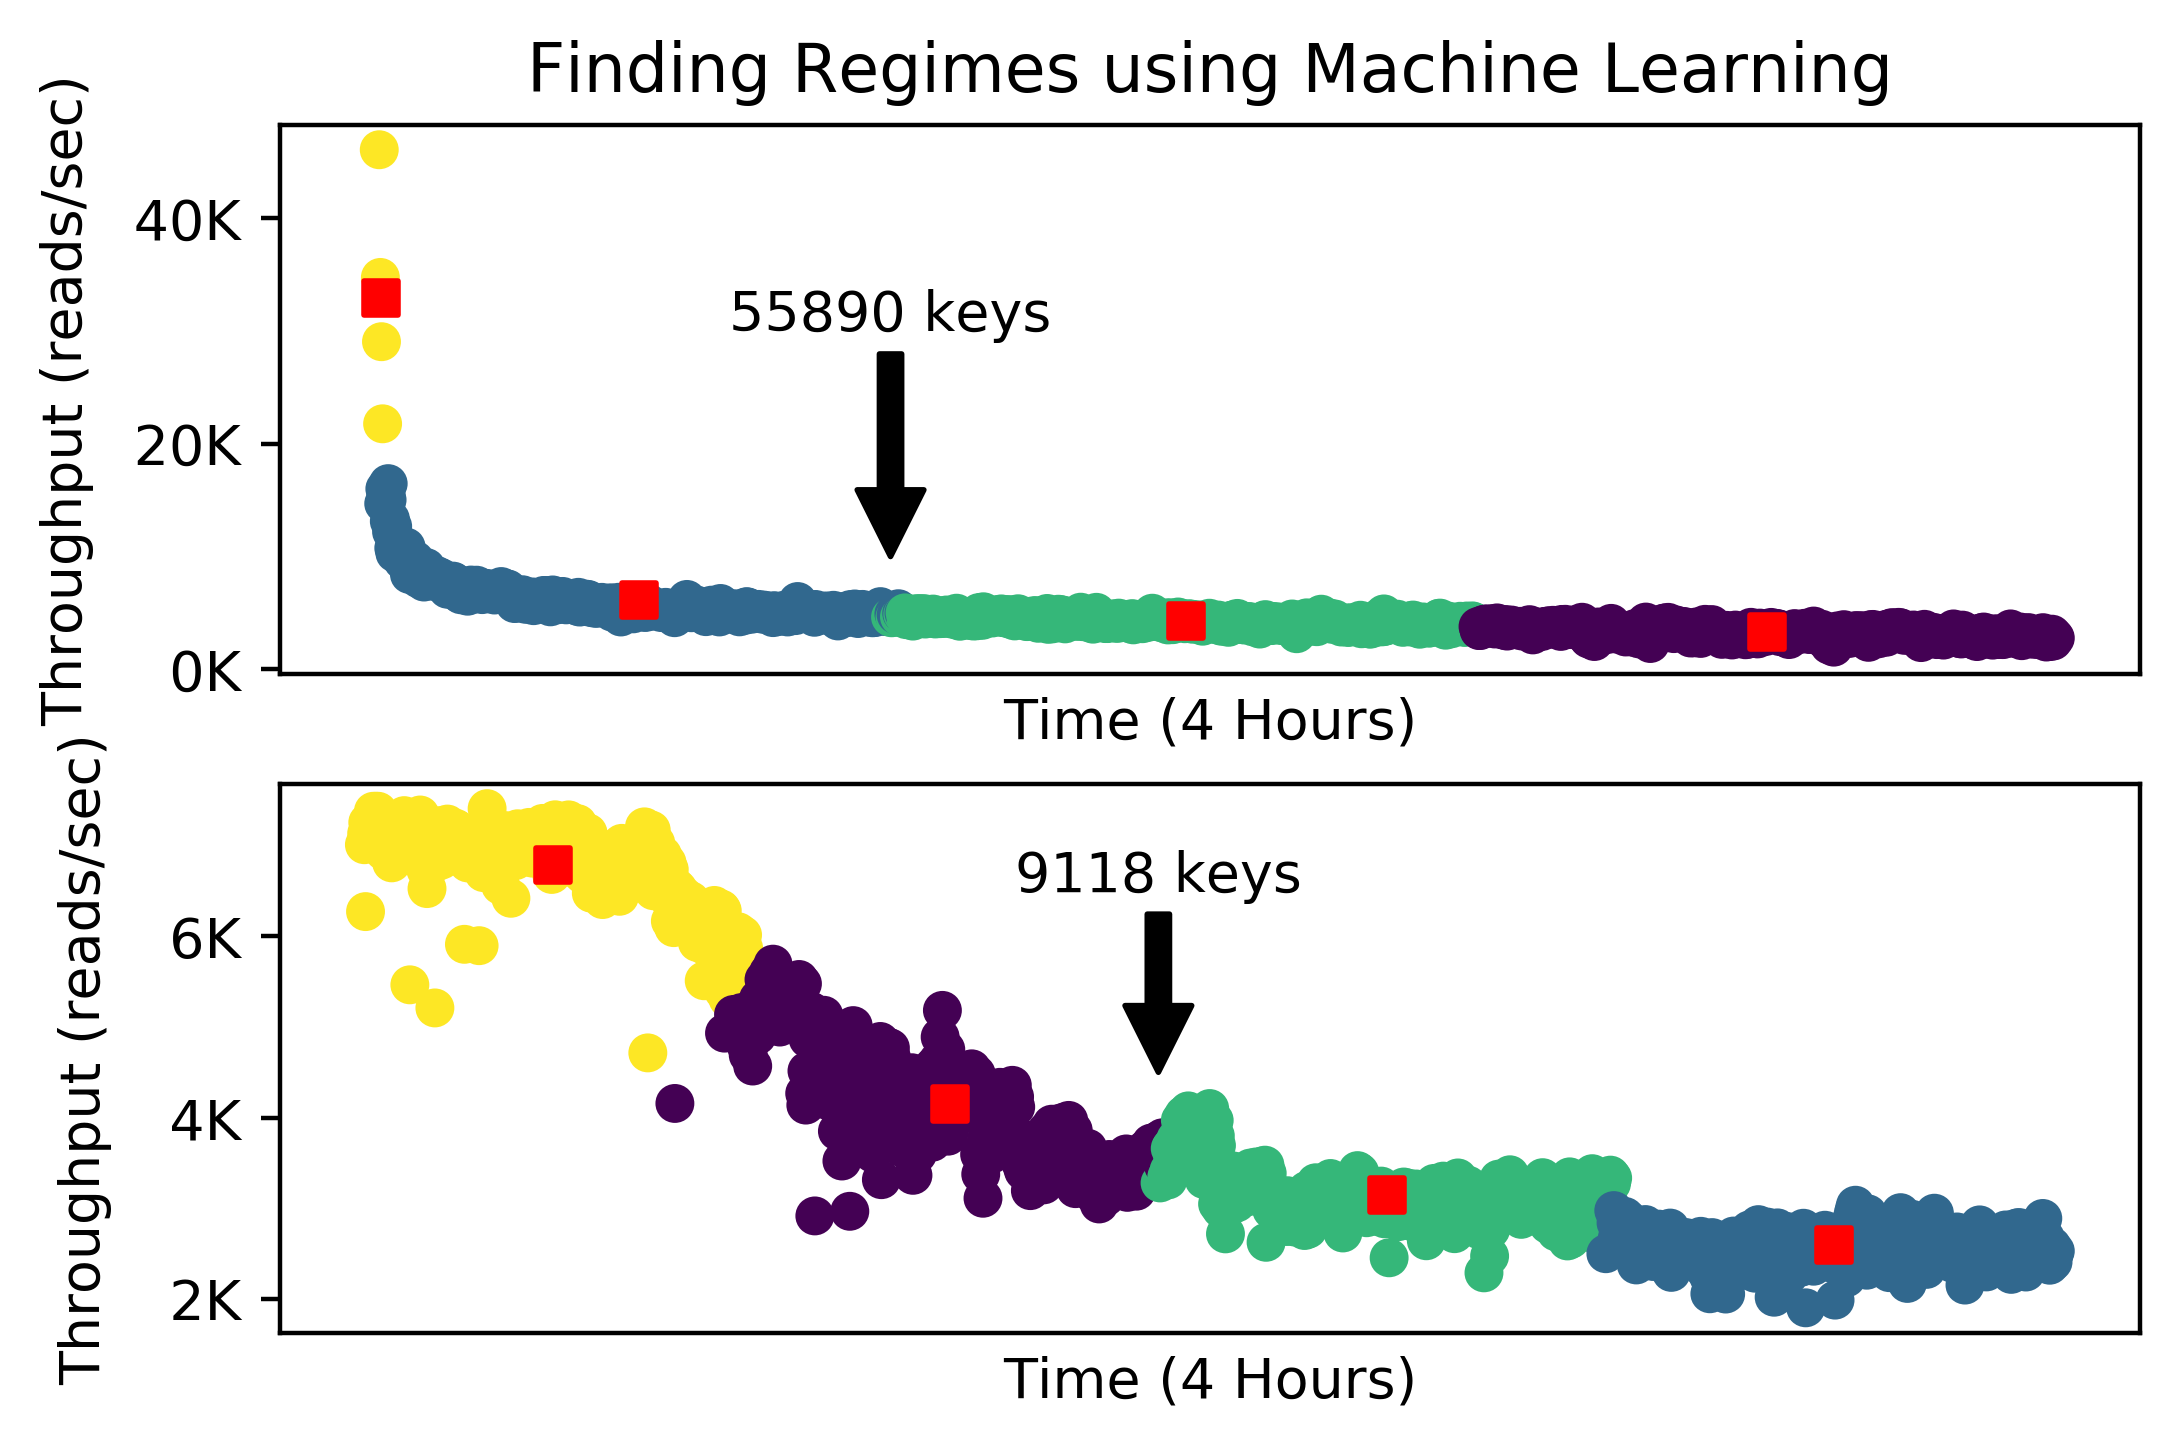
\includegraphics[width=0.5\textwidth]{figures/futurework-regimes.png}\\
  %\caption{Caching the 100 most recently accessed keys is sufficient for run 1
  %but more active keyspaces like run 0 need dynamic load balancing
  %policies.\label{fig:futurework-regimes}}
  \caption{The keyspace activity for Parsplice runs using two different growth 
  rates.  The blue line show the rate at which EOM minima values are retrieved
  from the Key-value store (y1 axis) and the black points show the number of
  unique minima keys accessed in a 1 second sliding window. 
  \label{fig:futurework-regimes}}
\end{figure}

The fine-grained data annotation capabilities provided by key-value storage is
a natural match for many types of scientific simulation. In simulations relying
on the finite element method, a mesh-based decomposition of a physical region
may result in millions or billions of mesh cells each containing materials,
pressures, temperatures and other characteristics that are required to
accurately simulate phenomena of interest. In our target application, a
molecular dynamics simulation named ParSplice~\cite{perez:jctc20150parsplice},
a key-value store is used to store both observed minima across a molecule's
equation of motion (EOM) and the hundreds or thousands of unique trajectories
calculated each second during a parallel job. Figure~\ref{fig:arch-parsplice}
shows the architecture of the ParSplice application.

In this paper we present a detailed analysis of how the ParSplice application
accesses EOM minima KV pairs over the course of a long running simulation
across a variety of initial conditions. Our analysis shows that small changes
to the rates at which new atoms enter the simulation, or the initial
temperature at which the simulation begins can have a strong effect on the
timing and frequency with which new EOM minima are discovered and referenced.

We also demonstrate the Mantle approach to load balancing for storage systems.
Although Mantle was intially developed for the Ceph distributed file system, the
flexible policy-based approach to load balancing provided by Mantle is also
applicable to the changing workloads generated by ParSplice. The Mantle
load-balancing API enables the storage system to change the active
load-balancing policy in use, a technique we will show is critical in
applications such as ParSplice that have multiple relatively stable and
relatively chaotic simulation regimes over the course of a long-running
simulation. Effectively, Mantle provides us the ability to choose among several
load-balancing policies as needed.

Finally, we explore the use of simple machine learning (ML) techniques to
identify "access regimes" within the ParSplice application's creation and
access of Key-Value pairs. The ML component of this work drives the Mantle
policy-switching API thus determining \emph{when} to change policies.

By understanding the regime-based key-value access patterns generated by
ParSplice, leveraging the dynamic load balancing capabilities of the Mantle
API, and using ML to identify Key-value access regime changes we are working
toward a flexible load balancing capability for software-defined storage
systems. 


%The storage of these small, computationally-intensive
%quantities is well suited to log-structured merge trees (LSM trees)
%that 
%a molecular dynamics simulation that relies on techniques for speculative
%execution a key-value store is used to capture both minima capture local and global minima across
%a molecules 
%The efficient, fine-grained annotation capabilities Key-value storage finds a natural match with scientific 
%The fine-grained annotation capabilities provided by Key-Value data
%organizations is of obvious benefit to scientific applications.

%The decomposition of physical domains into sma

%Mesh-based decomposition of
%physical regions of interest results in millions or billions of mesh cells
%each containing materials, pressures, temperatures and other characteristics
%that are required to accurately simulate phenomena of interest.  Although file
%formats are LSM Trees and Key-Value storage.  The popularity of LevelDB
%Advantages of Key-Value storage.
%  - Fine grain annotation
%  -
%
%Although the advantages of applying key-values
%The fine-grained Key-Value storage technology is 

%%% MSEVILLE
%Key-Value stores scale because they support (1) fine scale annotation and (2)
%flexible, extensible formats. Science applications are structured, entropy
%increases over time (e.g., Figure~\ref{fig:futurework-regimes} shows key
%distribution and key popularity changing over time). Our hypothesis is that
%re-distributing keys requires dynamic load balancing policies, similiar to
%distributed file systems.  A one-size-fits all policy is not sufficient. Our
%contributions are:


%% What is the problem?
%Load balancing is a useful tool for optimizing performance in systems that
%service highly accessed data\footnote{In this paper, we use the term ``data" to
%refer to the partitioned key-value pairs AND file system metadata.} but
%deciding how to make the migrations is a risky trade-off. In this paper, we
%show that a one-size-fits-all data load balancing policy is not sufficient for
%even the simplest of HPC applications and argue for a dynamic load balancing
%policy.
%
%% Explain techniques
%Resource migration is the key mechanism for load balancing. In storage, data
%can be distributed to alleviate overloaded servers or it can be concentrated to
%exploit locality. These techniques are at odds and selecting the wrong
%technique can have catastrophic consequences. For example, migrating data to an
%already overloaded server or increasing the network hops by spreading data
%across an underutilized cluster will impact performance negatively.
%
%% Why is concentration vs. distribution difficult?
%Unfortunately, deciding which optimization to use is difficult to reason about,
%especially with the scale and complexity of today's HPC architectures. While
%the mechanisms are usually built into the systems, the policies often times
%less refined and much more sensitive to the workload. So a system may have the
%ability exploit locality using techniques like bulk operations, multiple
%partition strategies, secondary indexes, and caching but deciding when, where,
%and how to use them is workload dependent and difficult to figure out.
%
%% What we did in the paper
%This paper takes an API designed to migrate file system metadata and applies it
%to an HPC key-value store.  The API helps control distribution and
%concentration by letting the administrator define how to migrate load, where to
%migrate load, and how much load to migrate. While designed for a different
%domains, this API encompasses many of the same properties we need for an HPC
%key-value store, namely:
%
%\begin{itemize}
%  \item services small/frequent requests
%  \item popularity drives distribution
%  \item locality drives concentration
%\end{itemize}
%
%\begin{figure}[t]
%  \noindent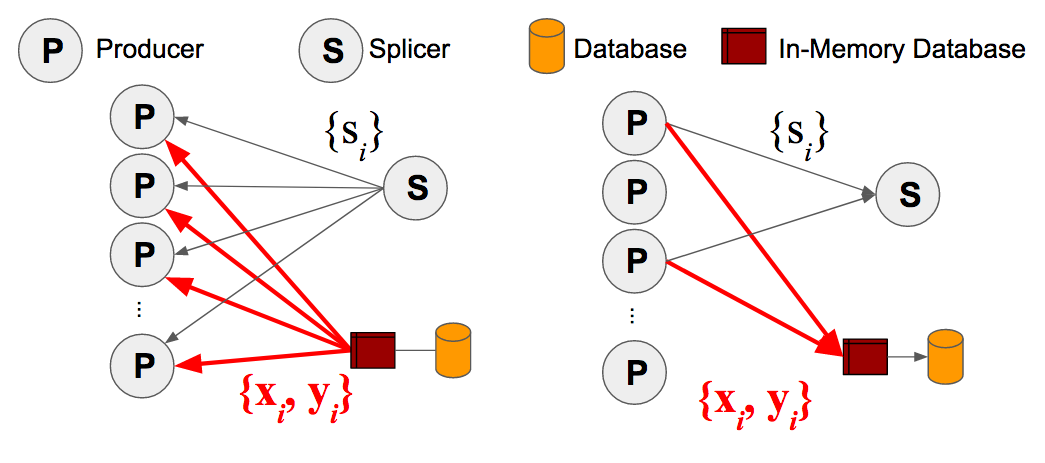
\includegraphics[width=19pc,angle=0]{figures/arch-parsplice.png}\\
%  \caption{ParSplice is a ready-heavy HPC application where producers use a
%  database for consistency. Replacing the single-node database with HXHIM
%  improves performance with load balancing.
%  \label{fig:arch-parsplice}}
%\end{figure}
%
%% Why is HXHIM a good fit?
%To show the efficacy of this approach, we examine the ParSplice molecular
%dynamics simulation application shown in Figure~\ref{fig:arch-parsplice}.
%ParSplice uses a single-node database for consistency, where producers, \(P\),
%push and pull coordinates, \{\(x_i, y_i\)\}, based on the segments,
%\{\(s_i\)\}, assigned by the splicer, \(S\). In this paper, we replace the
%database with a distributed key-value store designed for HPC enjoy performance
%optimizations for:
%
%\begin{itemize}
%  \item \texttt{put()} because of the distributed sync and load balancing based on:
%  \begin{itemize}
%    \item lazy synchronization with tombstones and RPCs
%    \item strong synchronization with consensus and blocking
%  \end{itemize}
%  \item \texttt{get()} because of the load balancing
%\end{itemize}
%
%It has 4 phases:
%
%\begin{enumerate}
%
%  \item splicer (S) tells producers (P) to compute segments for state \(s_i\)
%
%  \item P's pull initial coordinates \{\(x_i, y_i\)\} from database
%
%  \item a P inserts completed coordinates for segment \(s_i\) into database and
%  S broadcasts next segment(s) \(s_j\) 
%
%  \item P's pull new segment coordinates \{\(x_j, y_j\)\}
%\end{enumerate}
%
%, which has both a high computational footprint and data locality.
%The former suggests distribution to avoid hot spots while the latter encourages
%concentration to leverage the database's secondary indeices, bulk operations,
%and key redistribution functionality. 
%
%% Why is HXHIM a good fit?
%To show this approach at scale we study
%ParSplice~\cite{perez:jctc20150parsplice}, an HPC dynamics simulator that has
%both a high computation footprint, which suggests distribution to avoid hot
%spots, and data locality, which alternatively encourages concentration so the
%key-value store can use its functionality for secondary indices, bulk
%operations, and key redistribution. ParSplice uses both molecular dynamic (MD)
%and accelerated molecular dynamic methods (AMD) for simulations with long
%periods of inactivity and short periods of ``interesting" events.  Molecules in
%periods with many events are simulated with MD methods, which are exact but can
%only be run for a fixed, short period of time because the cumulative error
%grows so large. Alternatively, longer trajectories are simulated with AMD
%methods, which use statistics and parallelization to show the less precise
%state-to-tate trajectories. ParSplice tackles ``low-barrier problems", where
%the types of energy barriers separating states of the system are non-uniform
%(i.e. some require less energy than others). It chops long trajectories into
%parallelizable units called segments, where the segments can also be spliced
%together to form longer trajectories; this approach allows ParSplice to trade
%off accuracy for speed in a configurable way.
%
%% How is ParSplice implemented?
%ParSplice stores segments in a database while it runs. The splicer pastes
%segments generated by \(n\) producers.
%
%% What do we contribute?
%In this paper, we make the following contributions:
%
%\begin{enumerate}
%
%  \item protype that controls concentration and distribution using the bulk
%  operations, secondary indicies, and cursor types mechanisms
%  from~\cite{greenberg:hotstorage2015-mdhim}. 
%
%  \item quantifies benefits of server/client-side caching, many small messages,
%  and bulk operations.
%
%\end{enumerate}
